%!TeX root=../tese.tex
%("dica" para o editor de texto: este arquivo é parte de um documento maior)
% para saber mais: https://tex.stackexchange.com/q/78101/183146

% Apague as duas linhas abaixo (elas servem apenas para gerar um
% aviso no arquivo PDF quando não há nenhum dado a imprimir) e
% insira aqui o conteúdo dos apêndices do seu trabalho (ou deixe
% este arquivo vazio)

% \providecommand\aviso[1]{
  \clearpage
  \null
  \vfill
  \begin{hyphenrules}{nohyphenation}
    \centering\bfseries\Large
    #1\par
  \end{hyphenrules}
  \vfill
  \clearpage
}

\providecommand\avisoFolhasDeRosto{
  \aviso{
    {\huge Você precisa editar os arquivos no diretório ``\texttt{conteudo}''!}
    \par\bigskip\bigskip\bigskip\bigskip
    Para gerar a capa e demais páginas preliminares no formato correto,
    modifique os arquivos ``\texttt{conteudo/paginas-preliminares.tex}'' e
    ``\texttt{conteudo/metadados.tex}'', usando como base os arquivos
    correspondentes no diretório ``\texttt{conteudo-exemplo}''.
  }
}

\providecommand\avisoCapitulos{
  \aviso{
    Insira o conteúdo dos capítulos do seu trabalho no arquivo
    ``\texttt{capitulos.tex}'' do diretório ``\texttt{conteudo}''.
  }
}

\providecommand\avisoApendices{
  \aviso{
    Insira o conteúdo dos apêndices do seu trabalho no arquivo
    ``\texttt{apendices.tex}'' do diretório ``\texttt{conteudo}''
    (ou comente a linha correspondente em \texttt{tese.tex}).
  }
}

\providecommand\avisoAnexos{
  \aviso{
    Insira o conteúdo dos anexos do seu trabalho no arquivo
    ``\texttt{anexos.tex}'' do diretório ``\texttt{conteudo}''
    (ou comente a linha correspondente em \texttt{tese.tex}).
  }
}

% \avisoApendices
\chapter{Capturas de tela da aplicação}
\label{ap:prints}

\begin{figure}[H]
    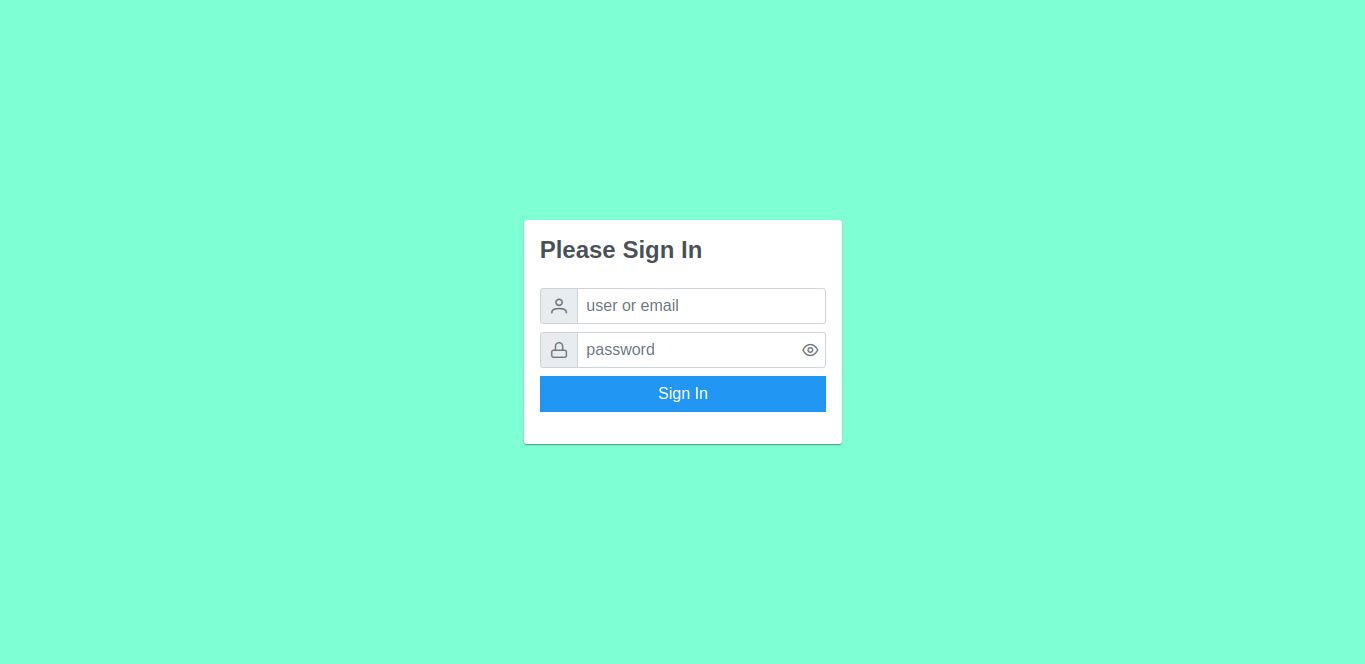
\includegraphics[scale=0.32]{figuras/vumos-interface-login.png}
    \caption{Captura de tela do \textit{vumos-interface} mostrando a página "Login"}
\end{figure}

\begin{figure}[H]
    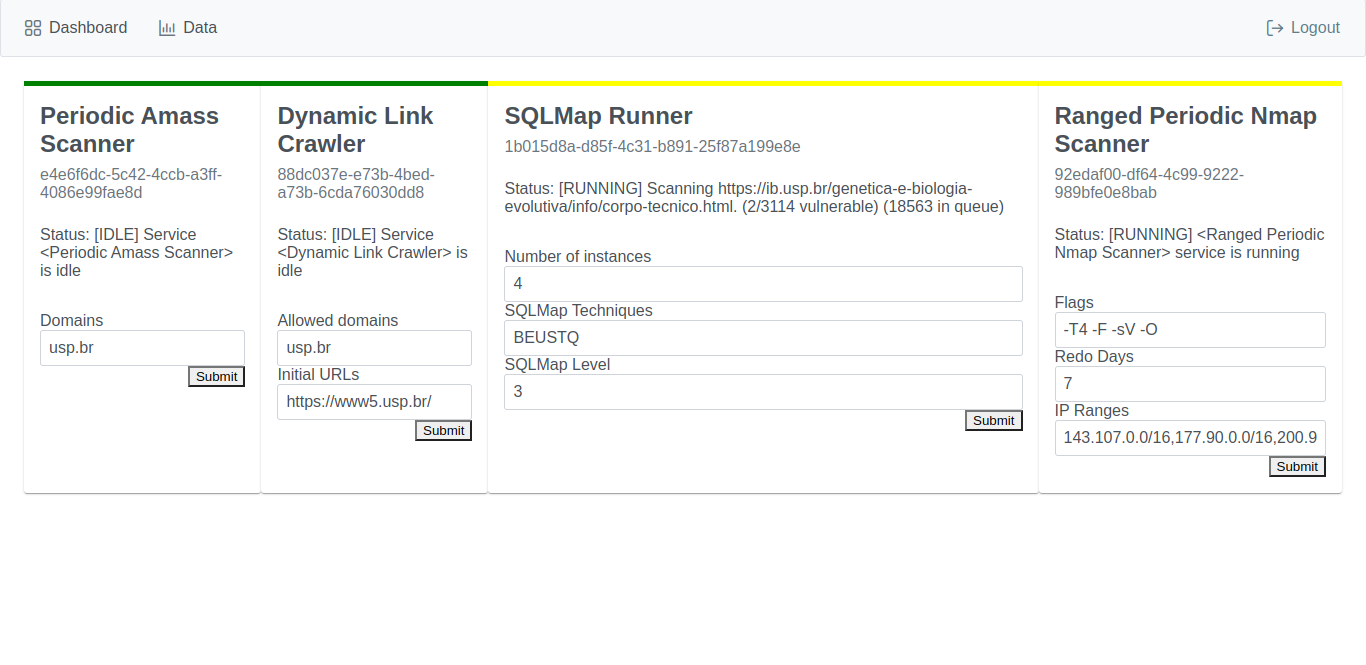
\includegraphics[scale=0.32]{figuras/vumos-interface-modules.png}
    \caption{Captura de tela do \textit{vumos-interface} mostrando a página "Dashboard"}
\end{figure}

\begin{figure}[H]
    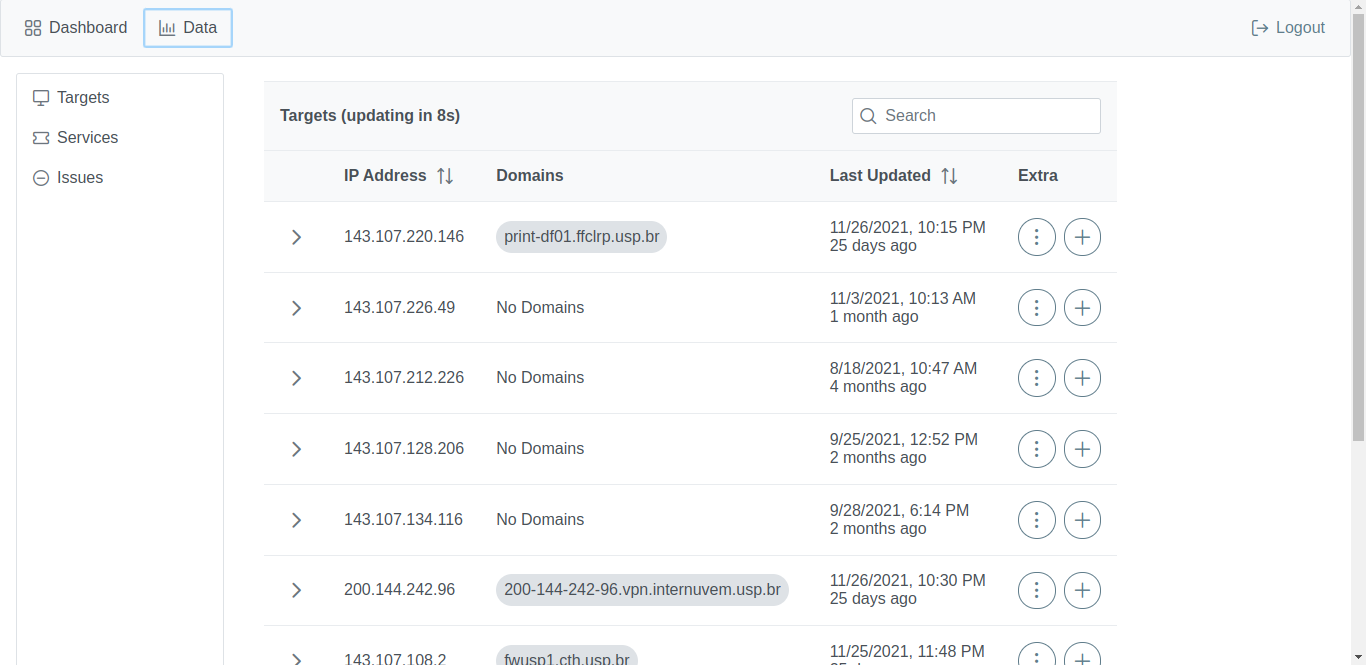
\includegraphics[scale=0.32]{figuras/vumos-interface-targets.png}
    \caption{Captura de tela do \textit{vumos-interface} mostrando a página "Targets"}
\end{figure}

\begin{figure}[H]
    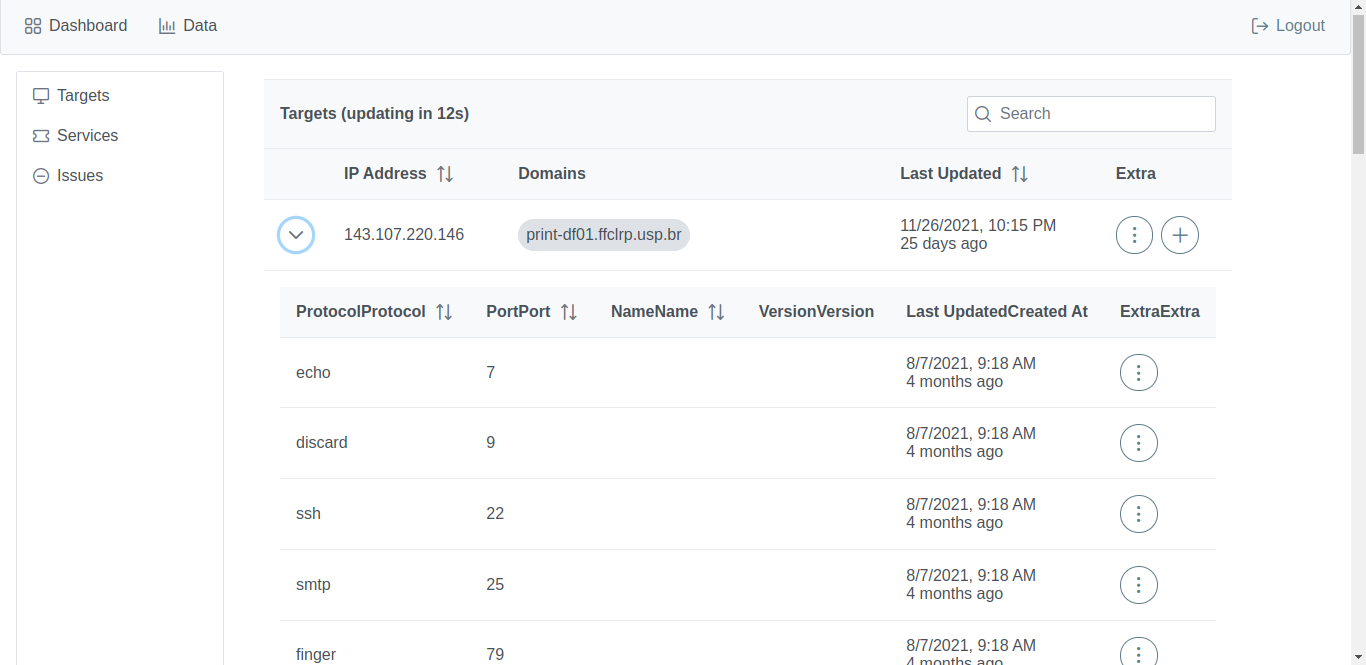
\includegraphics[scale=0.32]{figuras/vumos-interface-target-service.png}
    \caption{Captura de tela do \textit{vumos-interface} mostrando os serviços encontrados de um "Target" na página "Targets"}
\end{figure}

\begin{figure}[H]
    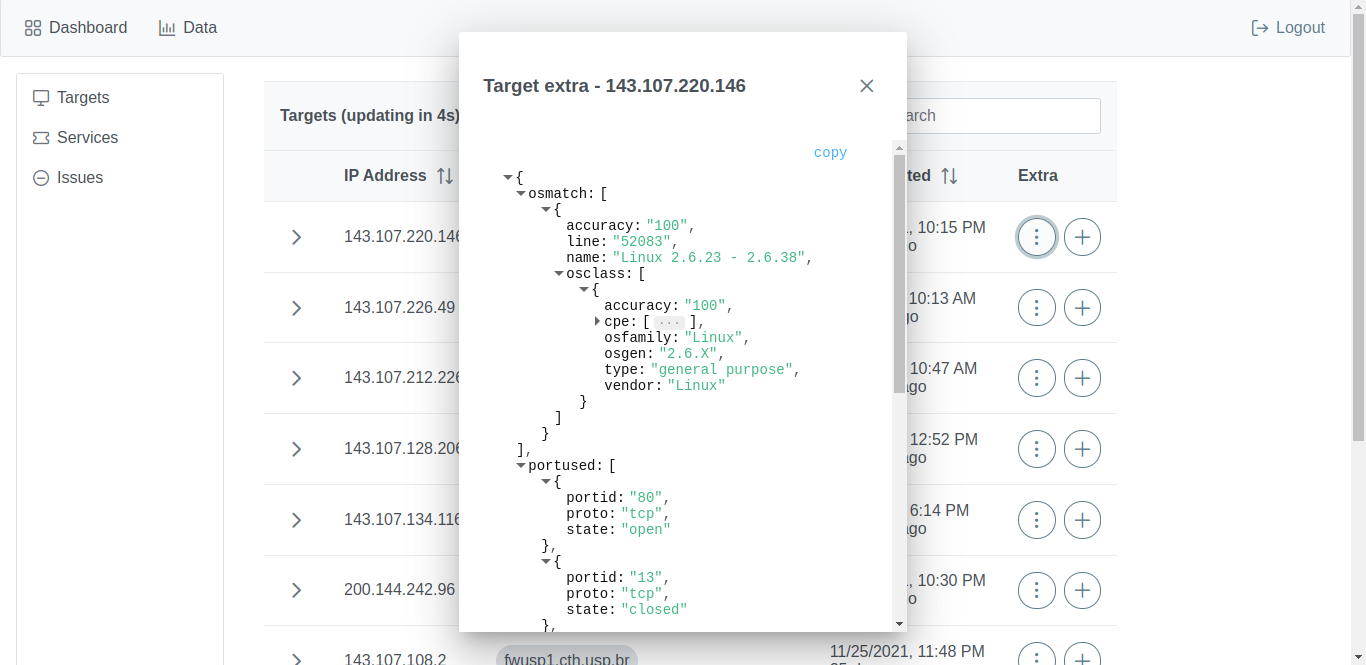
\includegraphics[scale=0.32]{figuras/vumos-interface-target-extra.png}
    \caption{Captura de tela do \textit{vumos-interface} mostrando os dados "extra" de uma entrada na página "Targets"}
\end{figure}

\begin{figure}[H]
    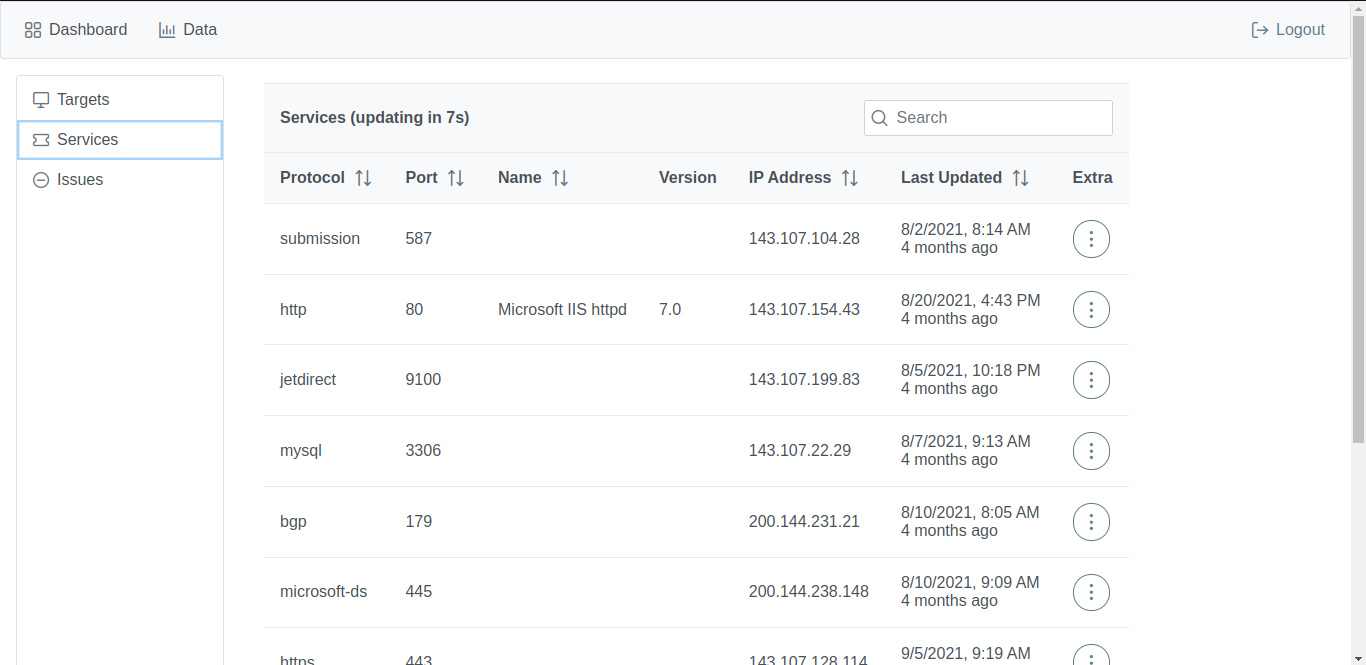
\includegraphics[scale=0.32]{figuras/vumos-interface-services.png}
    \caption{Captura de tela do \textit{vumos-interface} mostrando a página "Services"}
\end{figure}

\begin{figure}[H]
    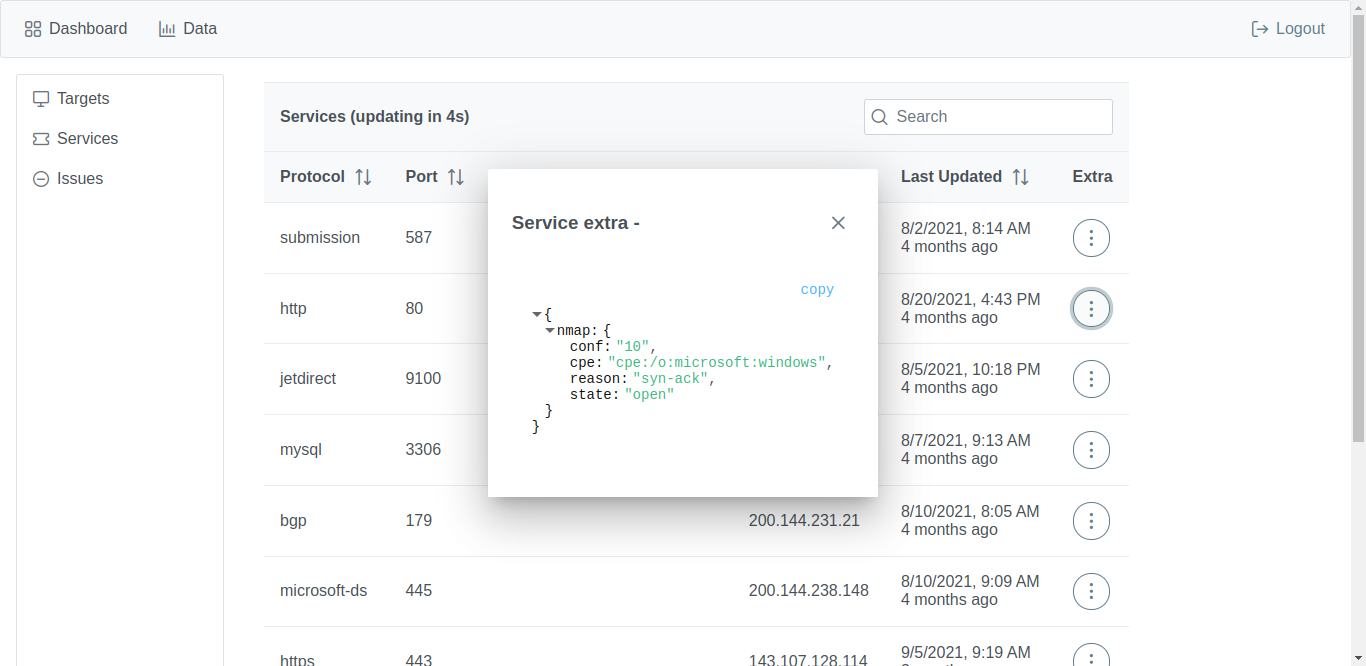
\includegraphics[scale=0.32]{figuras/vumos-interface-service-extra.png}
    \caption{Captura de tela do \textit{vumos-interface} mostrando os dados "extra" de uma entrada na página "Services"}
\end{figure}

\begin{figure}[H]
    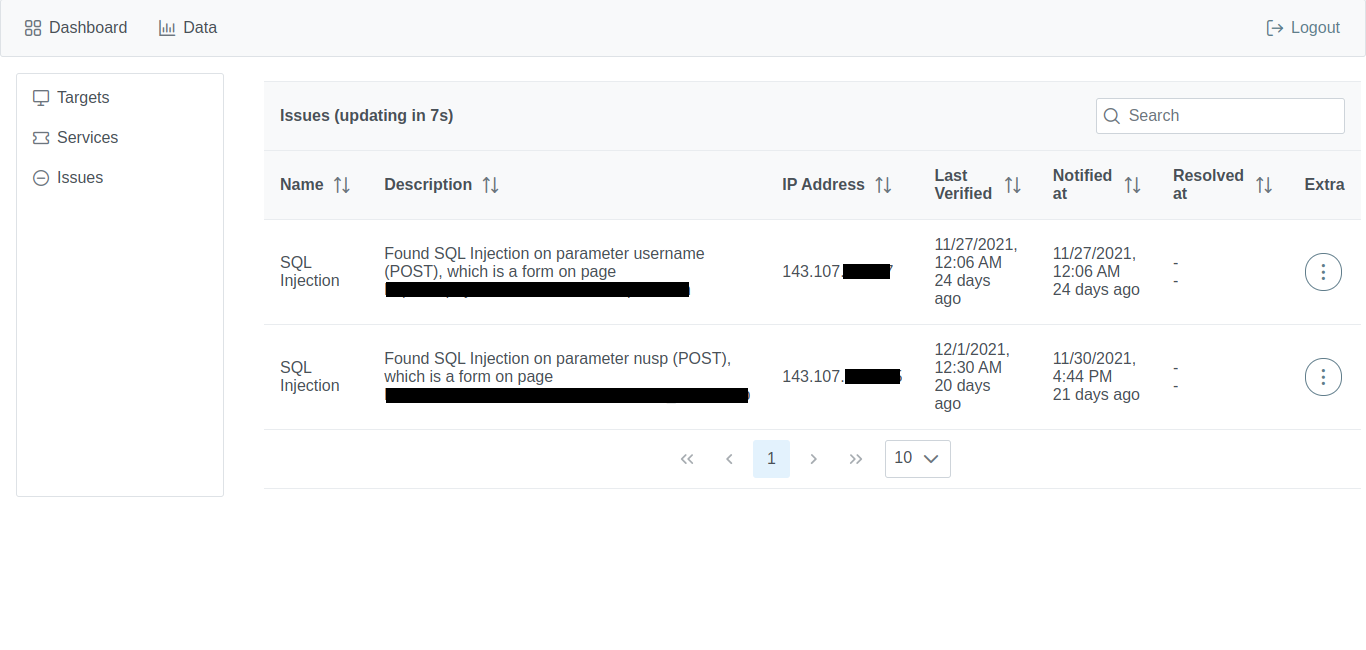
\includegraphics[scale=0.32]{figuras/vumos-interface-issues.png}
    \caption{Captura de tela do \textit{vumos-interface} mostrando a página "Issues". Alguns dados foram censurados para evitar expor os institutos afetados.}
\end{figure}


\begin{figure}[H]
    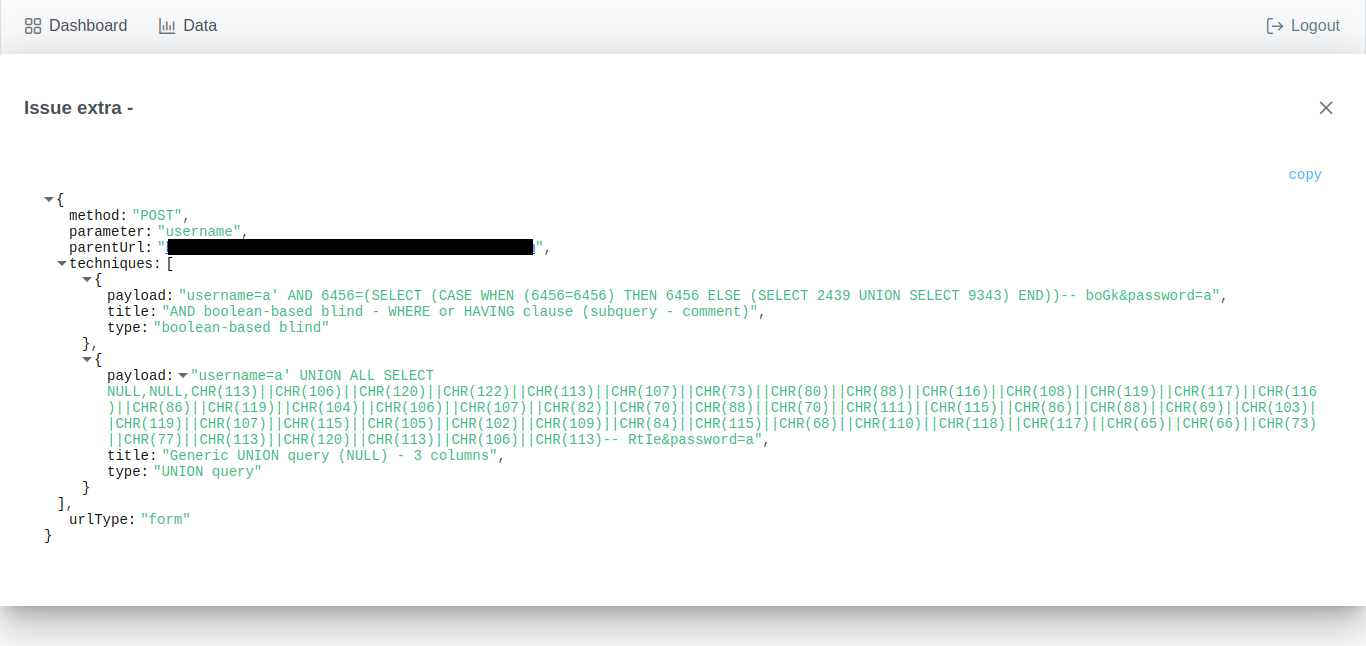
\includegraphics[scale=0.32]{figuras/vumos-interface-issue-extra.png}
    \caption{Captura de tela do \textit{vumos-interface} mostrando os dados "extra" de uma entrada na página "Issues". Alguns dados foram censurados para evitar expor os institutos afetados.}
\end{figure}
\par

% Os apêndices podem ser inseridos diretamente aqui ou "puxados" de outros
% arquivos.
% Em alguns (raros) casos, pode ser interessante usar \include ao
% invés de \input: https://tex.stackexchange.com/a/32058/183146

%\input{conteudo/...}
%\par
